\section{Image and Video Captioning}
\begin{frame}{}
    \LARGE Vision and Text Integration: \textbf{Image and Video Captioning}
\end{frame}

\begin{frame}[allowframebreaks]{What is Captioning?}
    \begin{itemize}
        \item \textbf{Definition:} Generating a descriptive text from an image or a video.
    \end{itemize}
    \begin{figure}
        \centering
        \fetchconvertimage{https://hips.hearstapps.com/popularmechanics/assets/16/38/1474656063-screen-shot-2016-09-23-at-24044-pm.png}{images/vision+text/captioning-1.png}{width=\textwidth,height=0.8\textheight,keepaspectratio}
    \end{figure}
\framebreak
    \begin{itemize}
        \item \textbf{Challenges:}
        \begin{itemize}
            \item Semantics
            \item Scene understanding
            \item Temporal context
        \end{itemize}
        \item \textbf{Applications:}
        \begin{itemize}
            \item Accessibility
            \item Content indexing
            \item Social media
            \item Surveillance
        \end{itemize}
    \end{itemize}
\end{frame}

\subsection{Image Captioning Pipeline}
\begin{frame}[allowframebreaks]{Image Captioning Pipeline}
    \begin{itemize}
        \item \textbf{Feature Extraction:} Use a CNN (e.g., ResNet) to extract visual features from the image.
        \item \textbf{Language Modeling:} Use an RNN, LSTM, or Transformer to generate a textual description based on the extracted features.
        \item \textbf{Encoder-Decoder Architecture:} The CNN acts as the encoder and the RNN/LSTM/Transformer as the decoder.
    \end{itemize}
    \begin{figure}
        \centering
        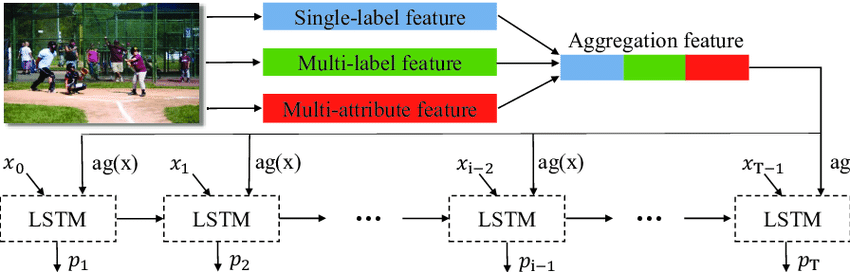
\includegraphics[width=0.8\textwidth]{images/vision+text/captioning-pipeline.png}
        \caption*{Typical image captioning pipeline.}
    \end{figure}
\framebreak
    \begin{figure}
        \centering
        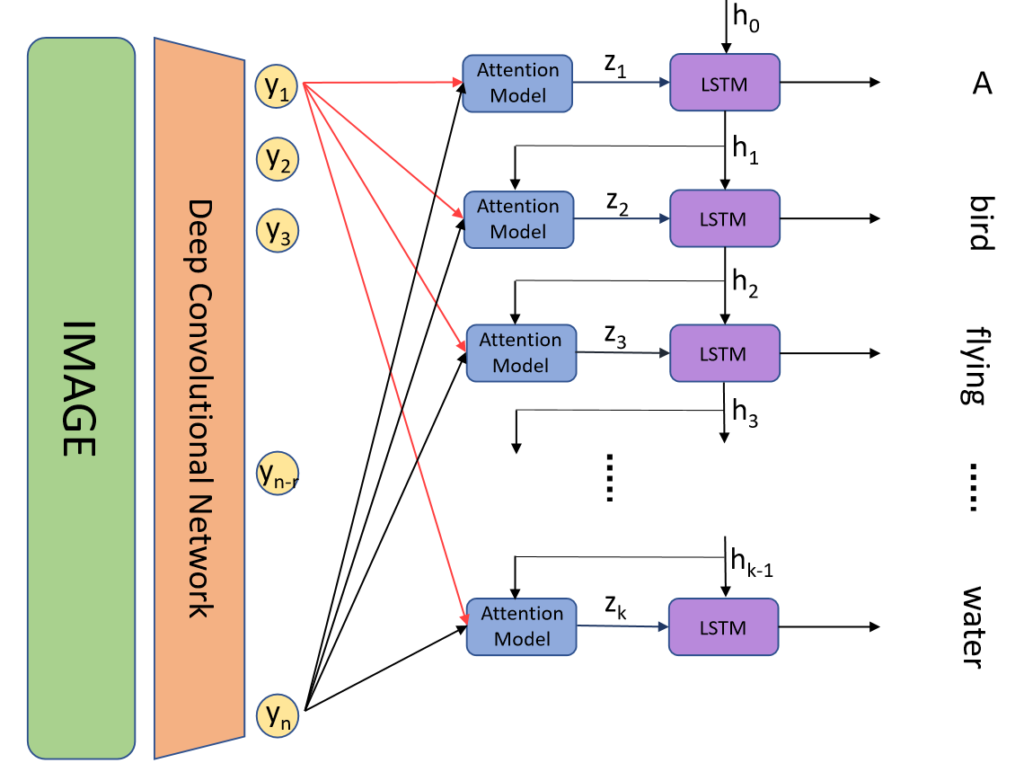
\includegraphics[width=0.8\textwidth,height=0.8\textheight,keepaspectratio]{images/vision+text/captioning-active-learning.png}
        \caption*{Active Learning in Image Captioning}
    \end{figure}
\end{frame}

\subsection{Show and Tell}
\begin{frame}[allowframebreaks]{Example: Show and Tell (Vinyals et al., 2015)}
    \begin{itemize}
        \item One of the first successful end-to-end image captioning models.
        \item Uses a CNN (Inception) as encoder and an LSTM as decoder.
        \item Trained to maximize the likelihood of the correct caption given the image.
    \end{itemize}
    \begin{figure}
        \centering
        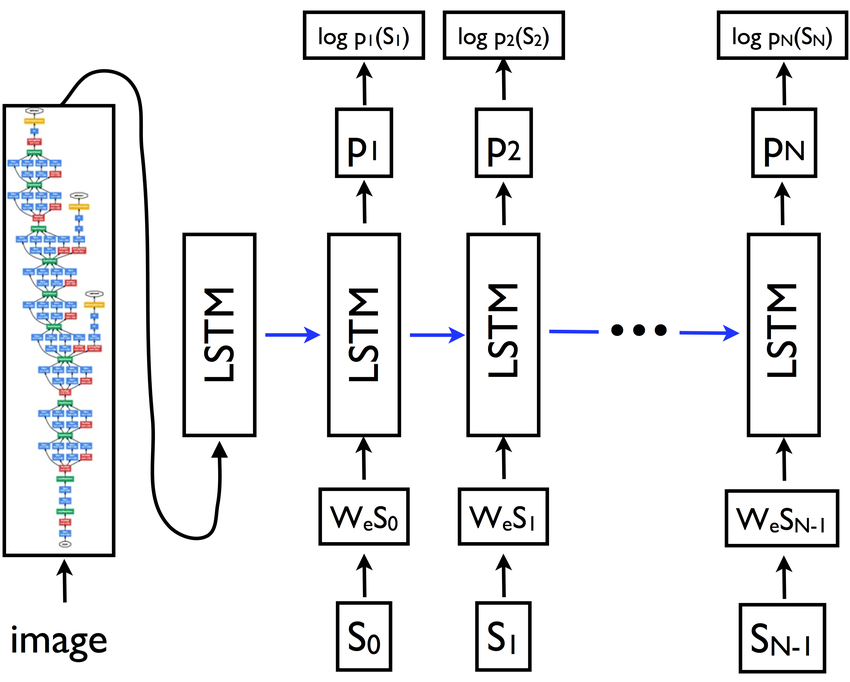
\includegraphics[width=\textwidth,height=0.8\textheight,keepaspectratio]{images/vision+text/show-and-tell.png}
        \caption*{Show and Tell model architecture (Vinyals et al., 2015).}
    \end{figure}
\framebreak
    \begin{figure}
        \centering
        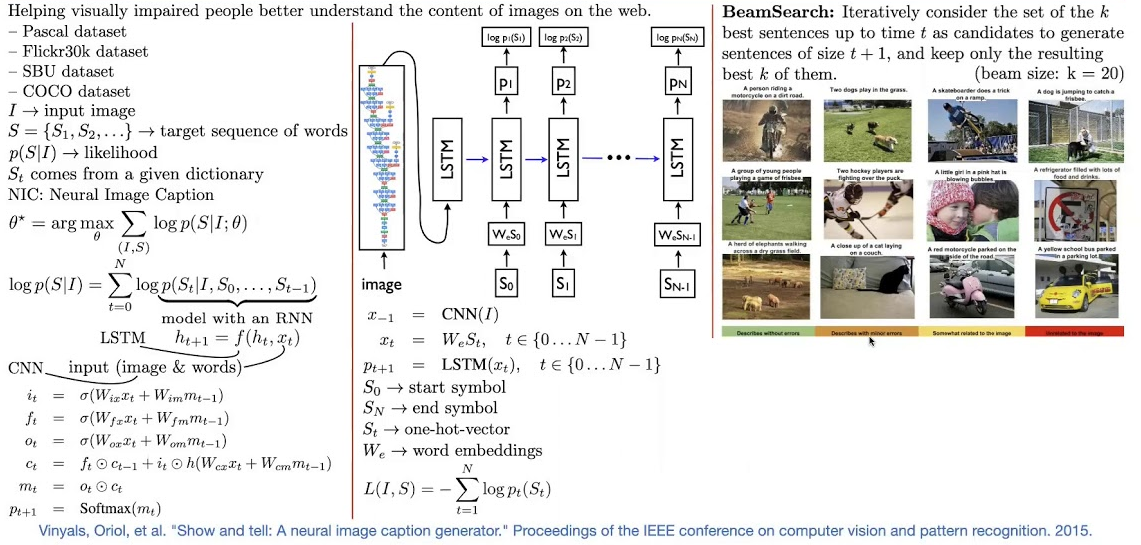
\includegraphics[width=1.08\textwidth,height=0.9\textheight,keepaspectratio]{images/vision+text/show-and-tell-2.png}
    \end{figure}
\framebreak
    \begin{figure}
        \centering
        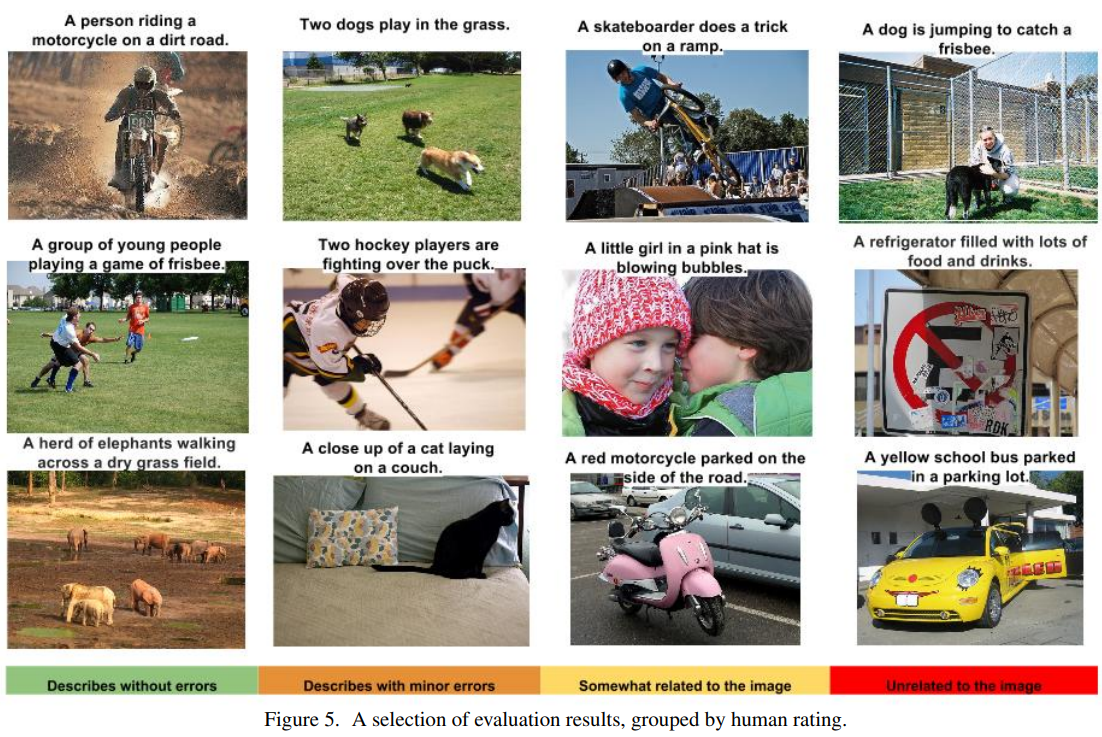
\includegraphics[width=1.08\textwidth,height=0.9\textheight,keepaspectratio]{images/vision+text/show-and-tell-result.png}
    \end{figure}
\end{frame}

\subsection{Video Captioning}
\begin{frame}[allowframebreaks]{Video Captioning}
    \begin{itemize}
        \item \textbf{Video Captioning:} Generating descriptive text for a sequence of video frames.
        \item \textbf{Temporal Sequence Modeling:} Adds modeling of temporal dependencies between frames, in addition to spatial features.
        \item \textbf{Common Architecture:} 
        \begin{itemize}
            \item CNN for frame-level feature extraction.
            \item RNN (e.g., LSTM/GRU) for modeling temporal sequence.
            \item Attention mechanisms to focus on relevant frames or regions.
        \end{itemize}
        \item \textbf{Recent Advances:}
        \begin{itemize}
            \item Transformer-based models for parallel sequence modeling.
            \item Memory networks for capturing long-term dependencies.
        \end{itemize}
    \end{itemize}
    \begin{figure}
        \centering
        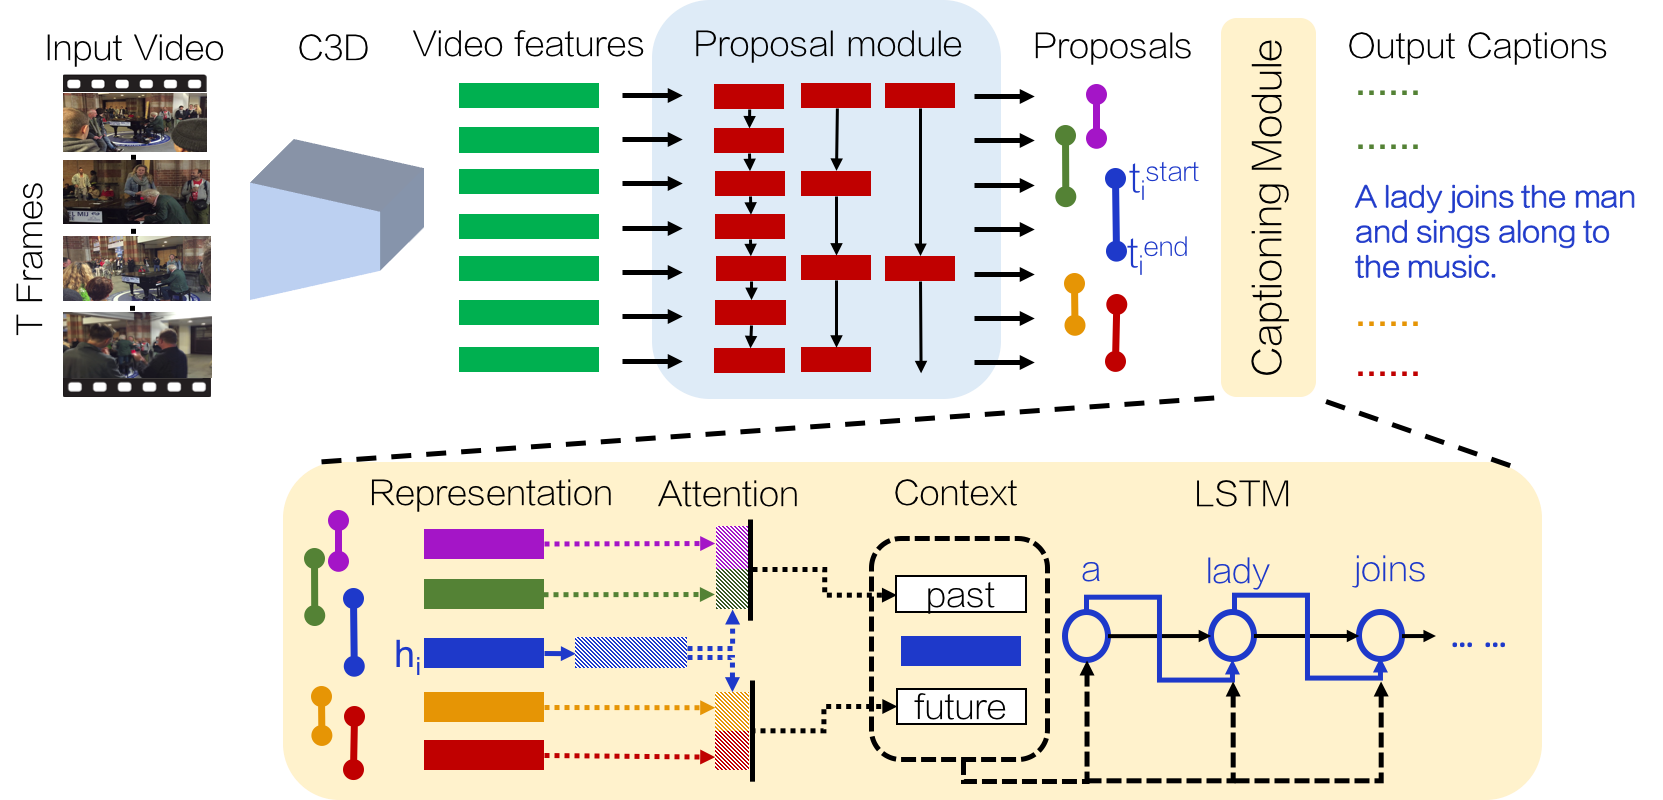
\includegraphics[width=0.85\textwidth]{images/vision+text/video-captioning-pipeline.png}
        \caption*{Dense-Captioning Events in Videos (Hendricks et al., 2017)}
    \end{figure}
\framebreak
    \begin{figure}
        \centering
        \fetchconvertimage{https://www.researchgate.net/publication/348510533/figure/fig2/AS:11431281179131504@1691159020381/DVC-Net-model-for-dense-video-captioning-DVC-dense-video-captioning.png}{images/vision+text/video-captioning-1.png}{width=\textwidth,height=0.9\textheight,keepaspectratio}
    \end{figure}
\framebreak
    \begin{figure}
        \centering
        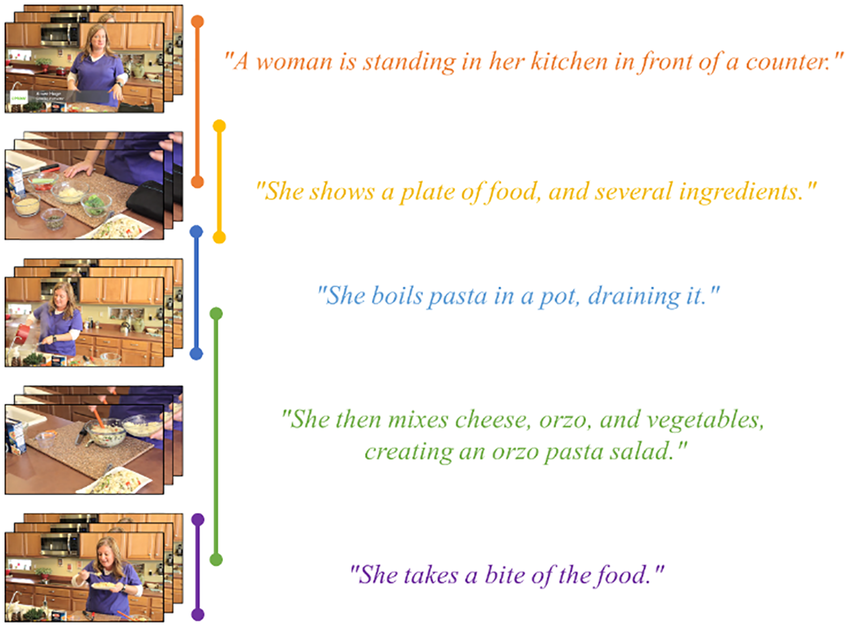
\includegraphics[width=0.85\textwidth]{images/vision+text/video-captioning-2.png}
    \end{figure}
\end{frame}

\subsection{Challenges in Captioning}
\begin{frame}[allowframebreaks]{Challenges in Captioning}
    \begin{itemize}
        \item \textbf{Ambiguity:} Multiple valid captions for the same image or video.
        \item \textbf{Context Understanding:} Captions need to capture context and semantics accurately.
        \item \textbf{Temporal Dynamics:} In video captioning, capturing the dynamics of actions and events over time is crucial.
        \item \textbf{Data Scarcity:} High-quality annotated datasets for training captioning models are limited.
        \item \textbf{Evaluation Metrics:} Evaluating caption quality is subjective and often relies on metrics like BLEU, METEOR, or CIDEr, which may not align with human judgment.
    \end{itemize}
\end{frame}
    

\subsection{Recent Advances and Datasets}
\begin{frame}[allowframebreaks]{Recent Advances in Captioning}
    \textbf{Image Captioning Advances:}
\framebreak
    \textbf{OSCAR:} Object-Semantics Aligned Pre-training for Vision-and-Language Tasks.
    \begin{figure}
        \centering
        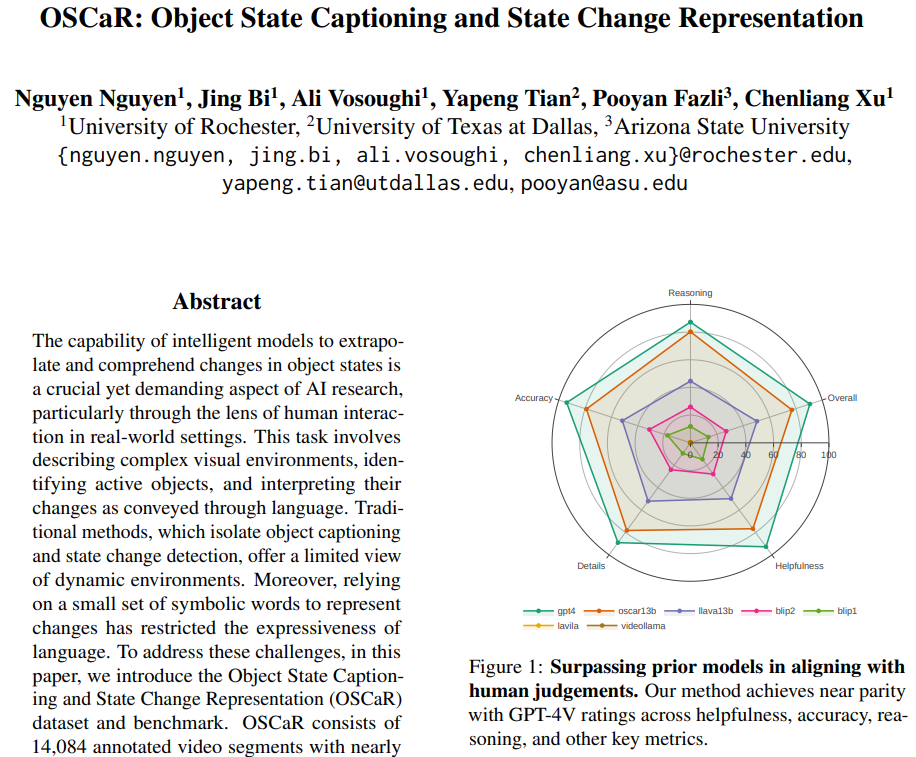
\includegraphics[width=1\textwidth,height=0.7\textheight,keepaspectratio]{images/vision+text/captioning-oscar.png}
    \end{figure}
\framebreak
    \textbf{OSCAR:} Object-Semantics Aligned Pre-training for Vision-and-Language Tasks.
    \begin{figure}
        \centering
        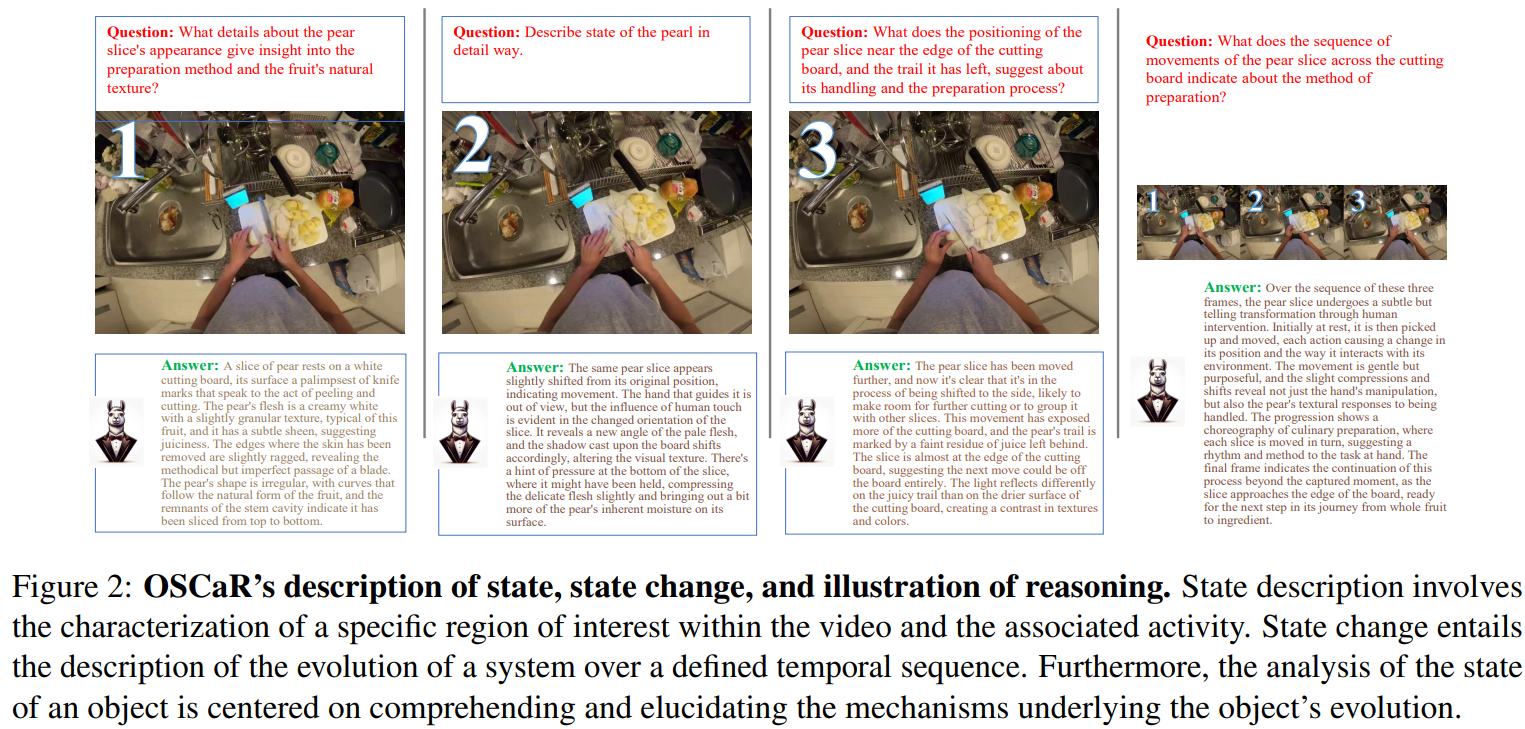
\includegraphics[width=1\textwidth,height=0.8\textheight,keepaspectratio]{images/vision+text/captioning-oscar-2.png}
    \end{figure}
\framebreak
    \textbf{VinVL:} Large-scale pre-training with improved object-visual representations.
    \begin{figure}
        \centering
        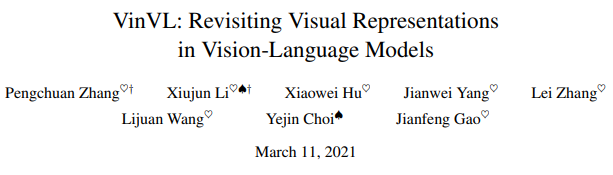
\includegraphics[width=1\textwidth,height=0.8\textheight,keepaspectratio]{images/vision+text/captioning-vinvl.png}
    \end{figure}
\framebreak
    \textbf{VinVL:} Large-scale pre-training with improved object-visual representations.
    \begin{figure}
        \centering
        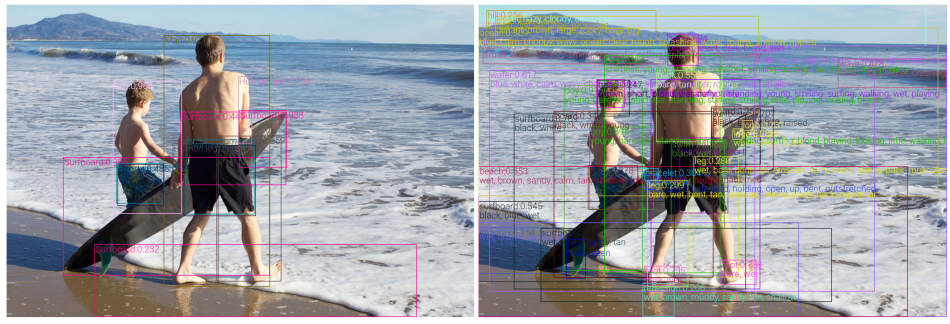
\includegraphics[width=1\textwidth,height=0.8\textheight,keepaspectratio]{images/vision+text/captioning-vinvl-2.png}
    \end{figure}
\framebreak
    \textbf{BLIP:} Bootstrapped Language-Image Pretraining for unified vision-language understanding and generation.
    \begin{figure}
        \centering
        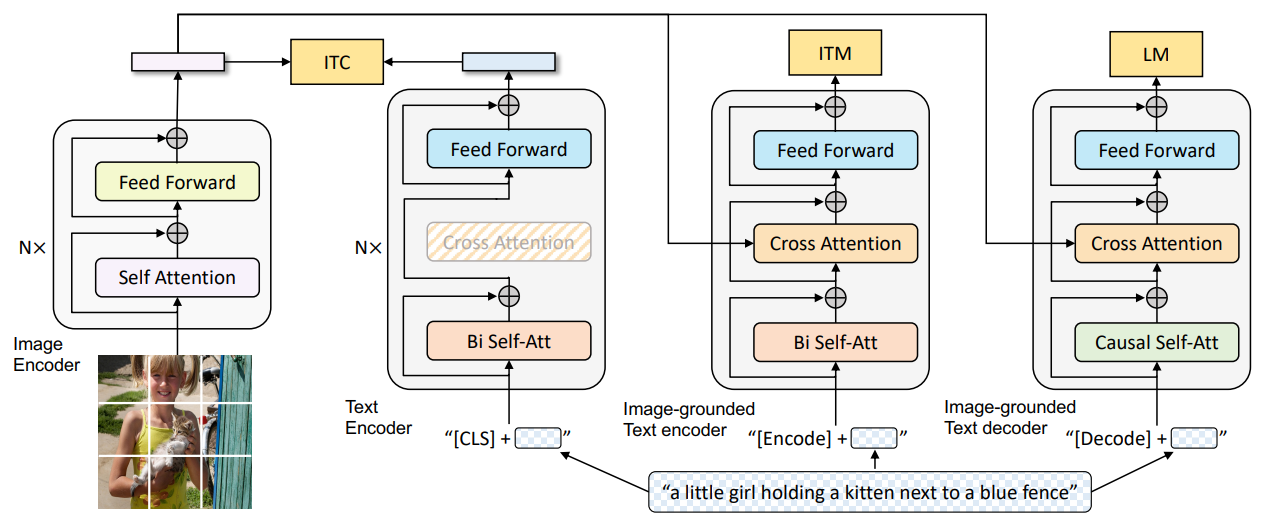
\includegraphics[width=1\textwidth,height=0.8\textheight,keepaspectratio]{images/vision+text/captioning-blip.png}
    \end{figure}
\framebreak
    \textbf{Video Captioning Advances:}
        \begin{itemize}
            \item \textbf{MARN:} Multi-modal Attentive Recurrent Network for video captioning.
            \item \textbf{STG-KD:} Spatio-Temporal Graph Knowledge Distillation for video captioning.
            \item \textbf{ClipCap:} Zero-shot image-to-text generation using CLIP and language models.
        \end{itemize}
\framebreak
    \textbf{Key Datasets}
        \begin{itemize}
            \item \textbf{MSCOCO:} Large-scale dataset for image captioning.
            \item \textbf{ActivityNet Captions:} Benchmark for dense video captioning.
            \item \textbf{YouCook2:} Large-scale dataset of instructional cooking videos with captions.
        \end{itemize}
\end{frame}
